
\documentclass[a4paper,12pt]{article}
\usepackage[utf8]{inputenc}
\usepackage[a4paper,
            bindingoffset=0.2in,
            left=1in,
            right=1in,
            top=1in,
            bottom=1in,
            footskip=.25in]{geometry}


%###############################################################################

%\input{~/layout/global_layout}


%###############################################################################

% packages begin

\usepackage[
  backend=biber,
  sortcites=true,
  style=alphabetic,
  eprint=true,
  backref=true
]{biblatex}
\addbibresource{bibliography.bib}

\usepackage{euscript}[mathcal]
% e.g. \mathcal{A} for fancy letters in mathmode
\usepackage{amsmath,amssymb,amstext,amsthm}

\usepackage{mdframed}
\newmdtheoremenv[nobreak=true]{problem}{Problem}[subsection]
\newmdtheoremenv[nobreak=true]{claim}{Claim}[subsection]
\newtheorem{definition}{Definition}[subsection]
\newtheorem{lemma}{Lemma}[claim]
\newtheorem{plemma}{Lemma}[problem]

\usepackage{mathtools}
\DeclarePairedDelimiter\ceil{\lceil}{\rceil}
\DeclarePairedDelimiter\floor{\lfloor}{\rfloor}

\usepackage{enumerate}
\usepackage[pdftex]{graphicx}
\usepackage{subcaption}
% 'draft' für schnelleres rendern mitübergeben -> [pdftex, draft]
% dadruch wird nicht das bild mitgerendered, sondern nur ein kasten mit bildname -> schont ressourcen

\usepackage{hyperref}

\usepackage{tikz}
\usetikzlibrary{arrows,automata,matrix,positioning,shapes}

% for adding non-formatted text to include source-code
\usepackage{listings}
\lstset{language=Python,basicstyle=\footnotesize}
% z.B.:
% \lstinputlisting{source_filename.py}
% \lstinputlisting[lanugage=Python, firstline=37, lastline=45]{source_filename.py}
%
% oder
%
% \begin{lstlisting}[frame=single]
% CODE HERE
%\end{lstlisting}
\usepackage{algorithm}
\usepackage{algpseudocode}

\usepackage{wasysym}

\usepackage{titling}
\usepackage{titlesec}
\usepackage[nocheck]{fancyhdr}
\usepackage{lastpage}

\usepackage{kantlipsum}
\usepackage[colorinlistoftodos,prependcaption,textsize=tiny]{todonotes}

% packages end
%###############################################################################

\pretitle{% add some rules
  \begin{center}
    \LARGE\bfseries
} %, make the fonts bigger, make the title (only) bold
\posttitle{%
  \end{center}%
  %\vskip .75em plus .25em minus .25em% increase the vertical spacing a bit, make this particular glue stretchier
}
\predate{%
  \begin{center}
    \normalsize
}
\postdate{%
  \end{center}%
}

\titleformat*{\section}{\Large\bfseries}
\titleformat*{\subsection}{\large\bfseries}
\titleformat*{\subsubsection}{\normalsize\bfseries}

\titleformat*{\paragraph}{\Large\bfseries}
\titleformat*{\subparagraph}{\large\bfseries}

%###############################################################################
% TODO define Headers and Fotter

\pagestyle{fancy}
\fancyhf{}
% l=left, c=center, r=right; e=even_pagenumber, o=odd_pagenumber; h=header, f=footer
% example: [lh] -> left header, [lof,ref] -> fotter left when odd, right when even
%\fancyhf[lh]{}
%\fancyhf[ch]{}
%\fancyhf[rh]{}
%\fancyhf[lf]{}
\fancyhf[cf]{\footnotesize Page \thepage\ of \pageref*{LastPage}}
%\fancyhf[rf]{}
\renewcommand{\headrule}{} % removes horizontal header line

% Fotter options for first page

\fancypagestyle{firstpagestyle}{
  \renewcommand{\thedate}{\textmd{}} % removes horizontal header line
  \fancyhf{}
  \fancyhf[lh]{\ttfamily M.Sc. Computer Science\\KTH Royal Institute of Technology}
  \fancyhf[rh]{\ttfamily Period 3\\\today}
  \fancyfoot[C]{\footnotesize Page \thepage\ of \pageref*{LastPage}}
  \renewcommand{\headrule}{} % removes horizontal header line
}
%###############################################################################
% Todo: define Title

\title{
  \normalsize{DD2358 VT25 Introduction to}\\
  \normalsize{High Performance Computing}\\
  \large{Assignment 3 - Using Compilation Techniques and GPUs for Optimization}\\
}
\author{
  \small Rishi Vijayvargiya\\[-0.75ex]
%  \footnotesize\texttt{MN: }\\[-1ex]
  \scriptsize\texttt{rishiv@kth.se}
  \and
  \small Lennart Herud\\[-0.75ex]
%  \footnotesize\texttt{MN: }\\[-1ex]
  \scriptsize\texttt{herud@kth.se}
  \and
  \small Paul Mayer\\[-0.75ex]
%  \footnotesize\texttt{MN: }\\[-1ex]
  \scriptsize\texttt{pmayer@kth.se}
  \and
  \small Adrian Sušec\\[-0.75ex]
%  \footnotesize\texttt{MN: }\\[-1ex]
  \scriptsize\texttt{susec@kth.se}
}
\date{}

%###############################################################################
% define Commands

\newcommand{\N}{\mathbb{N}}
\newcommand{\R}{\mathbb{R}}
\newcommand{\Z}{\mathbb{Z}}
\newcommand{\I}{\mathbb{I}}

\newcommand{\E}{\mathbb{E}}
\newcommand{\Prob}{\mathbb{P}}

\renewcommand{\epsilon}{\varepsilon}

% Todo: Set Counter to Excercise Sheet Number
\setcounter{section}{3}
\setcounter{subsection}{0}

%###############################################################################
%###############################################################################

\begin{document}
\maketitle
\thispagestyle{firstpagestyle}

% \tableofcontents
\listoftodos

\vspace{1em}

%---
%
\section*{Prefix}
\todo[inline]{Make sure title and headers are correctly changed!}
\todo[inline]{Change counter to match excercise sheet}

% content begin
%

\subsection*{Code Repository}
The code for this assignment can be found in the following github repository: \url{https://github.com/paulmyr/DD2358-HPC25/tree/master/03_compgpu}.

\subsection{Gauss-Seidel for Poisson Solver}
\subsubsection{Develop the Gauss-Seidel solver with NumPy}
\todo[inline]{Plot the performance varying the grid size}
\subsubsection{Profiling Code using lineprofiler}
\begin{lstlisting}[language=bash,basicstyle=\tiny\ttfamily]
Total time: 62.731 s
File: .\03_compgpu\exercise1\poisson_solver.py
Function: numpy_pure_gauss_seidel at line 8

Line #      Hits         Time  Per Hit   % Time  Line Contents
==============================================================
     8                                           @profile
     9                                           def numpy_pure_gauss_seidel(f):
    10      5000      33409.1      6.7      0.1      newf = f.copy()
    11
    12    243000      93182.7      0.4      0.1      for i in range(1,newf.shape[0]-1):
    13  21090000    8332316.0      0.4     13.3          for j in range(1,newf.shape[1]-1):
    14  62556000   35721824.4      0.6     56.9              newf[i,j] = 0.25 * (newf[i,j+1] + newf[i,j-1] +
    15  41704000   18544127.1      0.4     29.6                                  newf[i+1,j] + newf[i-1,j])
    16
    17      5000       6168.0      1.2      0.0      return newf

Total time: 99.7621 s
\end{lstlisting}


\subsubsection{Use the Cython Annotation tool to identify the bottleneck}
\subsubsection{Use Cython to optimize}

\subsubsection{Use PyTorch to port your code to Nvidia GPUs}
We implement the task in the file \verb|torch_cupy.ipynb|. The code is ported to torch equivalent to the previous diffusion task
where the loops were replaced by \verb|np.roll| operations. We adapted the code as specified in the task description by calculating the
updated field value using the array of the previous iteration, which result in a slower convergence, but enables us to parallelize the field calculations
instead of sequential calculations in case of in field operations.

To port the resulting code to torch, we use the equivalent torch function \verb|torch.roll| and reset the edge values to zero after each iteration. We use the same utility functions as for the numpy code.
Necessary adaptions were made to the input grid, as the datatype needs to be a \verb|torch.tensor| and the object will be assigned to the GPU using the \verb|.cuda()| method.

\subsubsection{Use CuPy to port your code to Nvidia GPUs}
We did the same initial steps as for the torch implementation:
We implement the task in the file \verb|torch_cupy.ipynb|. The code is ported to torch equivalent to the previous diffusion task
where the loops were replaced by \verb|np.roll| operations. We adapted the code as specified in the task description by calculating the
updated field value using the array of the previous iteration, which result in a slower convergence, but enables us to parallelize the field calculations
instead of sequential calculations in case of in field operations.

To port the resulting code to cupy, we use the equivalent torch function \verb|cupy.roll| and reset the edge values to zero after each iteration. We use the same utility functions as for the numpy code.
Necessary adaptions were made to the input grid, as the datatype needs to be a \verb|cupy.array| and the call \verb|cupy.cuda.Stream.null.synchronize()| ensures a GPU execution which is finished before returning the function result.

\subsubsection{Measure the performance (execution time) with GPU}
Before testing the performance, we added test cases to ensure correct execution of the implementations.
The test cases proved a valid implementation and can be found in the notebook as well.

The results of our performance measurements can be seen below.
\begin{figure}[H]
  \centering
  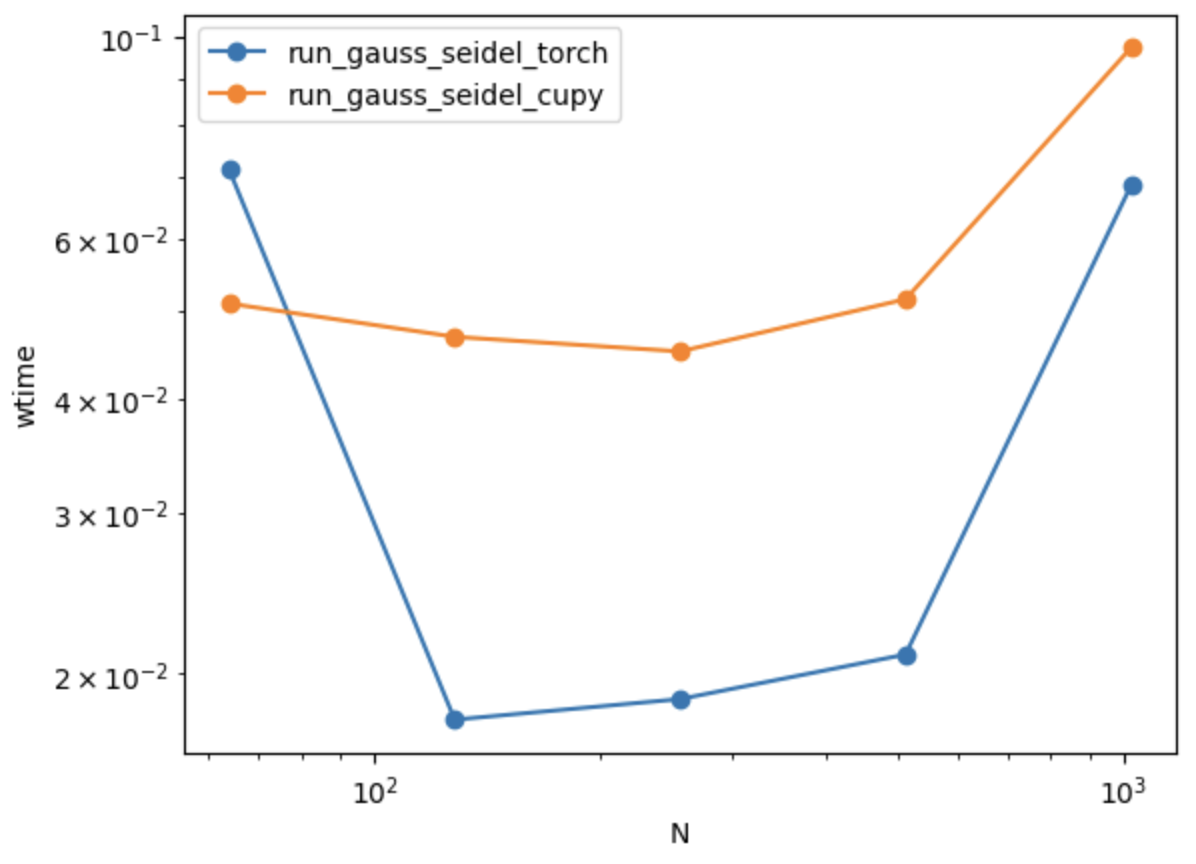
\includegraphics[width=0.8\textwidth]{images/cupy_torch_gpu.png}
  \caption{Running Time Comparisons For Different Grid Sizes (Log-Scale)}
\end{figure}

 Interestingly the running time of the torch implementation seems to be more efficient for large Arrays, while it is
 inferior to the cupy implementation for small Array sizes.

\subsubsection{Save the newgrid matrix as an hdf5 file using h5py }
We interpreted the task as saving the torch and cupy implementation results. We saved the torch and cupy calculations over a grid with size \verb|N = 1024|
as dict entries in a \verb|hdf5| file in the repository (see \verb|matrix_gpu.hdf5|).

\subsection{Bonus: Fast Fractal Fun with Cython \& GPUs}
The original Mandelbrot Set code provided in the assignment description can be found in the \verb|mandelbrot_set_default.py| file in the code-repository (\href{https://github.com/paulmyr/DD2358-HPC25/blob/master/03_compgpu/bonus/mandelbrot_set_default.py}{link}). The code to display the generated Mandelbrot Set has been commented out to allow for \verb|pytests| to be run against the file. All other code files related to the Bonus (mentioned or not mentioned in this report) can be found in the \verb|bonus/| directory of the code-repository.

\subsubsection{Cython Optimization of Baseline}
To optimize the code with \verb|Cython|, we first examined the key areas where a large number of calls were being made to the Python virtual machine. For this, we extracted the \verb|mandelbrot| and the \verb|mandelbrot_set| functions from the original file into the file \verb|cython_mandelbrot.pyx| and then ran the \verb|cython -a cython_mandelbrot.pyx| command. 

\verb|og_cython_mandelbrot.html| was the resulting HTML file and is present in the code-repository. Below we include a screenshot of the file

\begin{figure}[H]
  \centering
  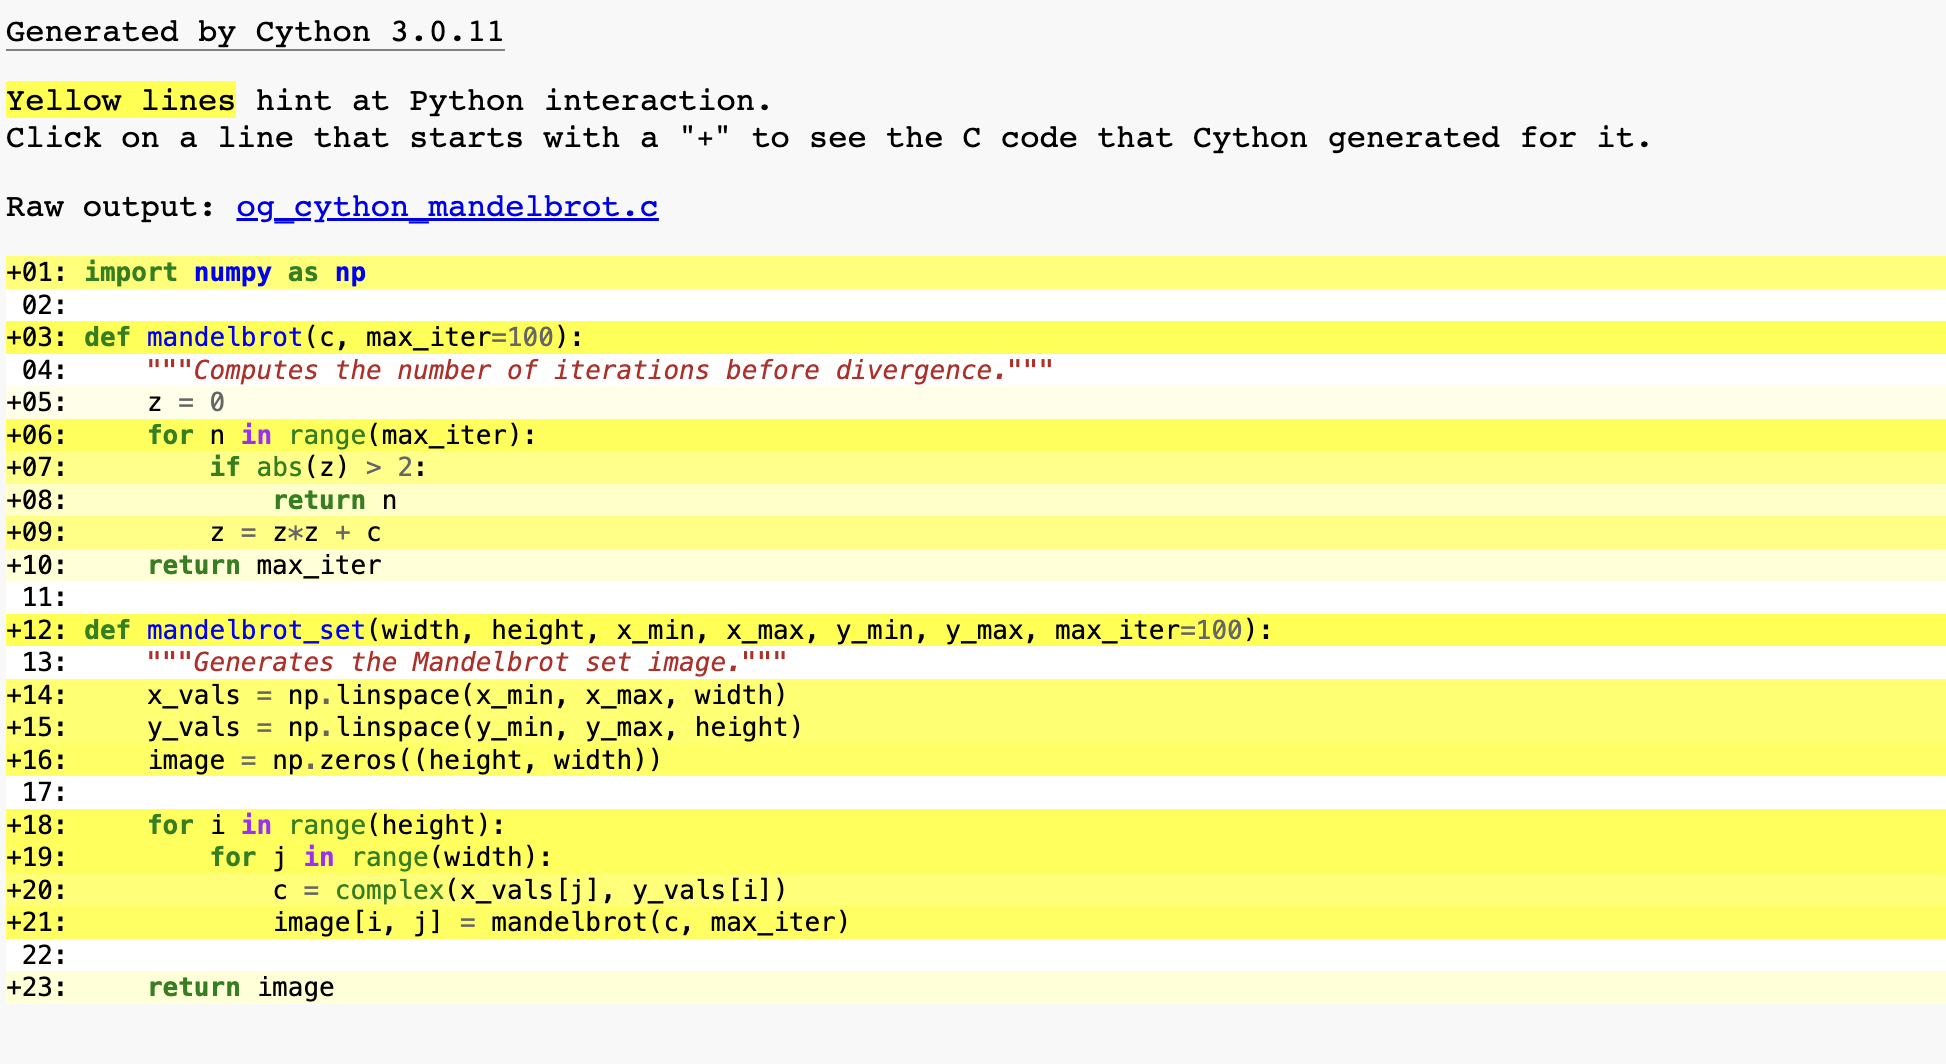
\includegraphics[width=0.8\textwidth]{images/og_mandelbrot_cython.png}
  \caption{Python VM Calls in the Original Mandelbrot Code}
\end{figure}

After this, we added type annotations to the parameters and the local variables of the functions \verb|mandelbrot| and \verb|mandelbrot_set|. We also used \underline{typed memory views} instead of Numpy arrays for the \verb|x_vals, y_vals, image| variables in the \verb|mandelbrot_set| function. Additionally, since the calculations for array addressing in the code are automatic (in the form of a counter of a loop within the bounds of the arrays), we also \underline{disabled bounds checking} for both the functions. We anticipated that this should have a noticeable impact for the \verb|mandelbrot_set| function. This is because in that function, we are using nested loops for iteration: so disabling bounds checking could make the inner loop iterations faster (thus making the outer loop iterations faster as well). 

We then included the required building/setup code in \verb|setup.py| and used the command \verb|python3 setup.py build_ext --inplace| to get the \verb|.so| and \verb|.c| files (also present in the code repository for reference). 

\begin{figure}[H]
  \centering
  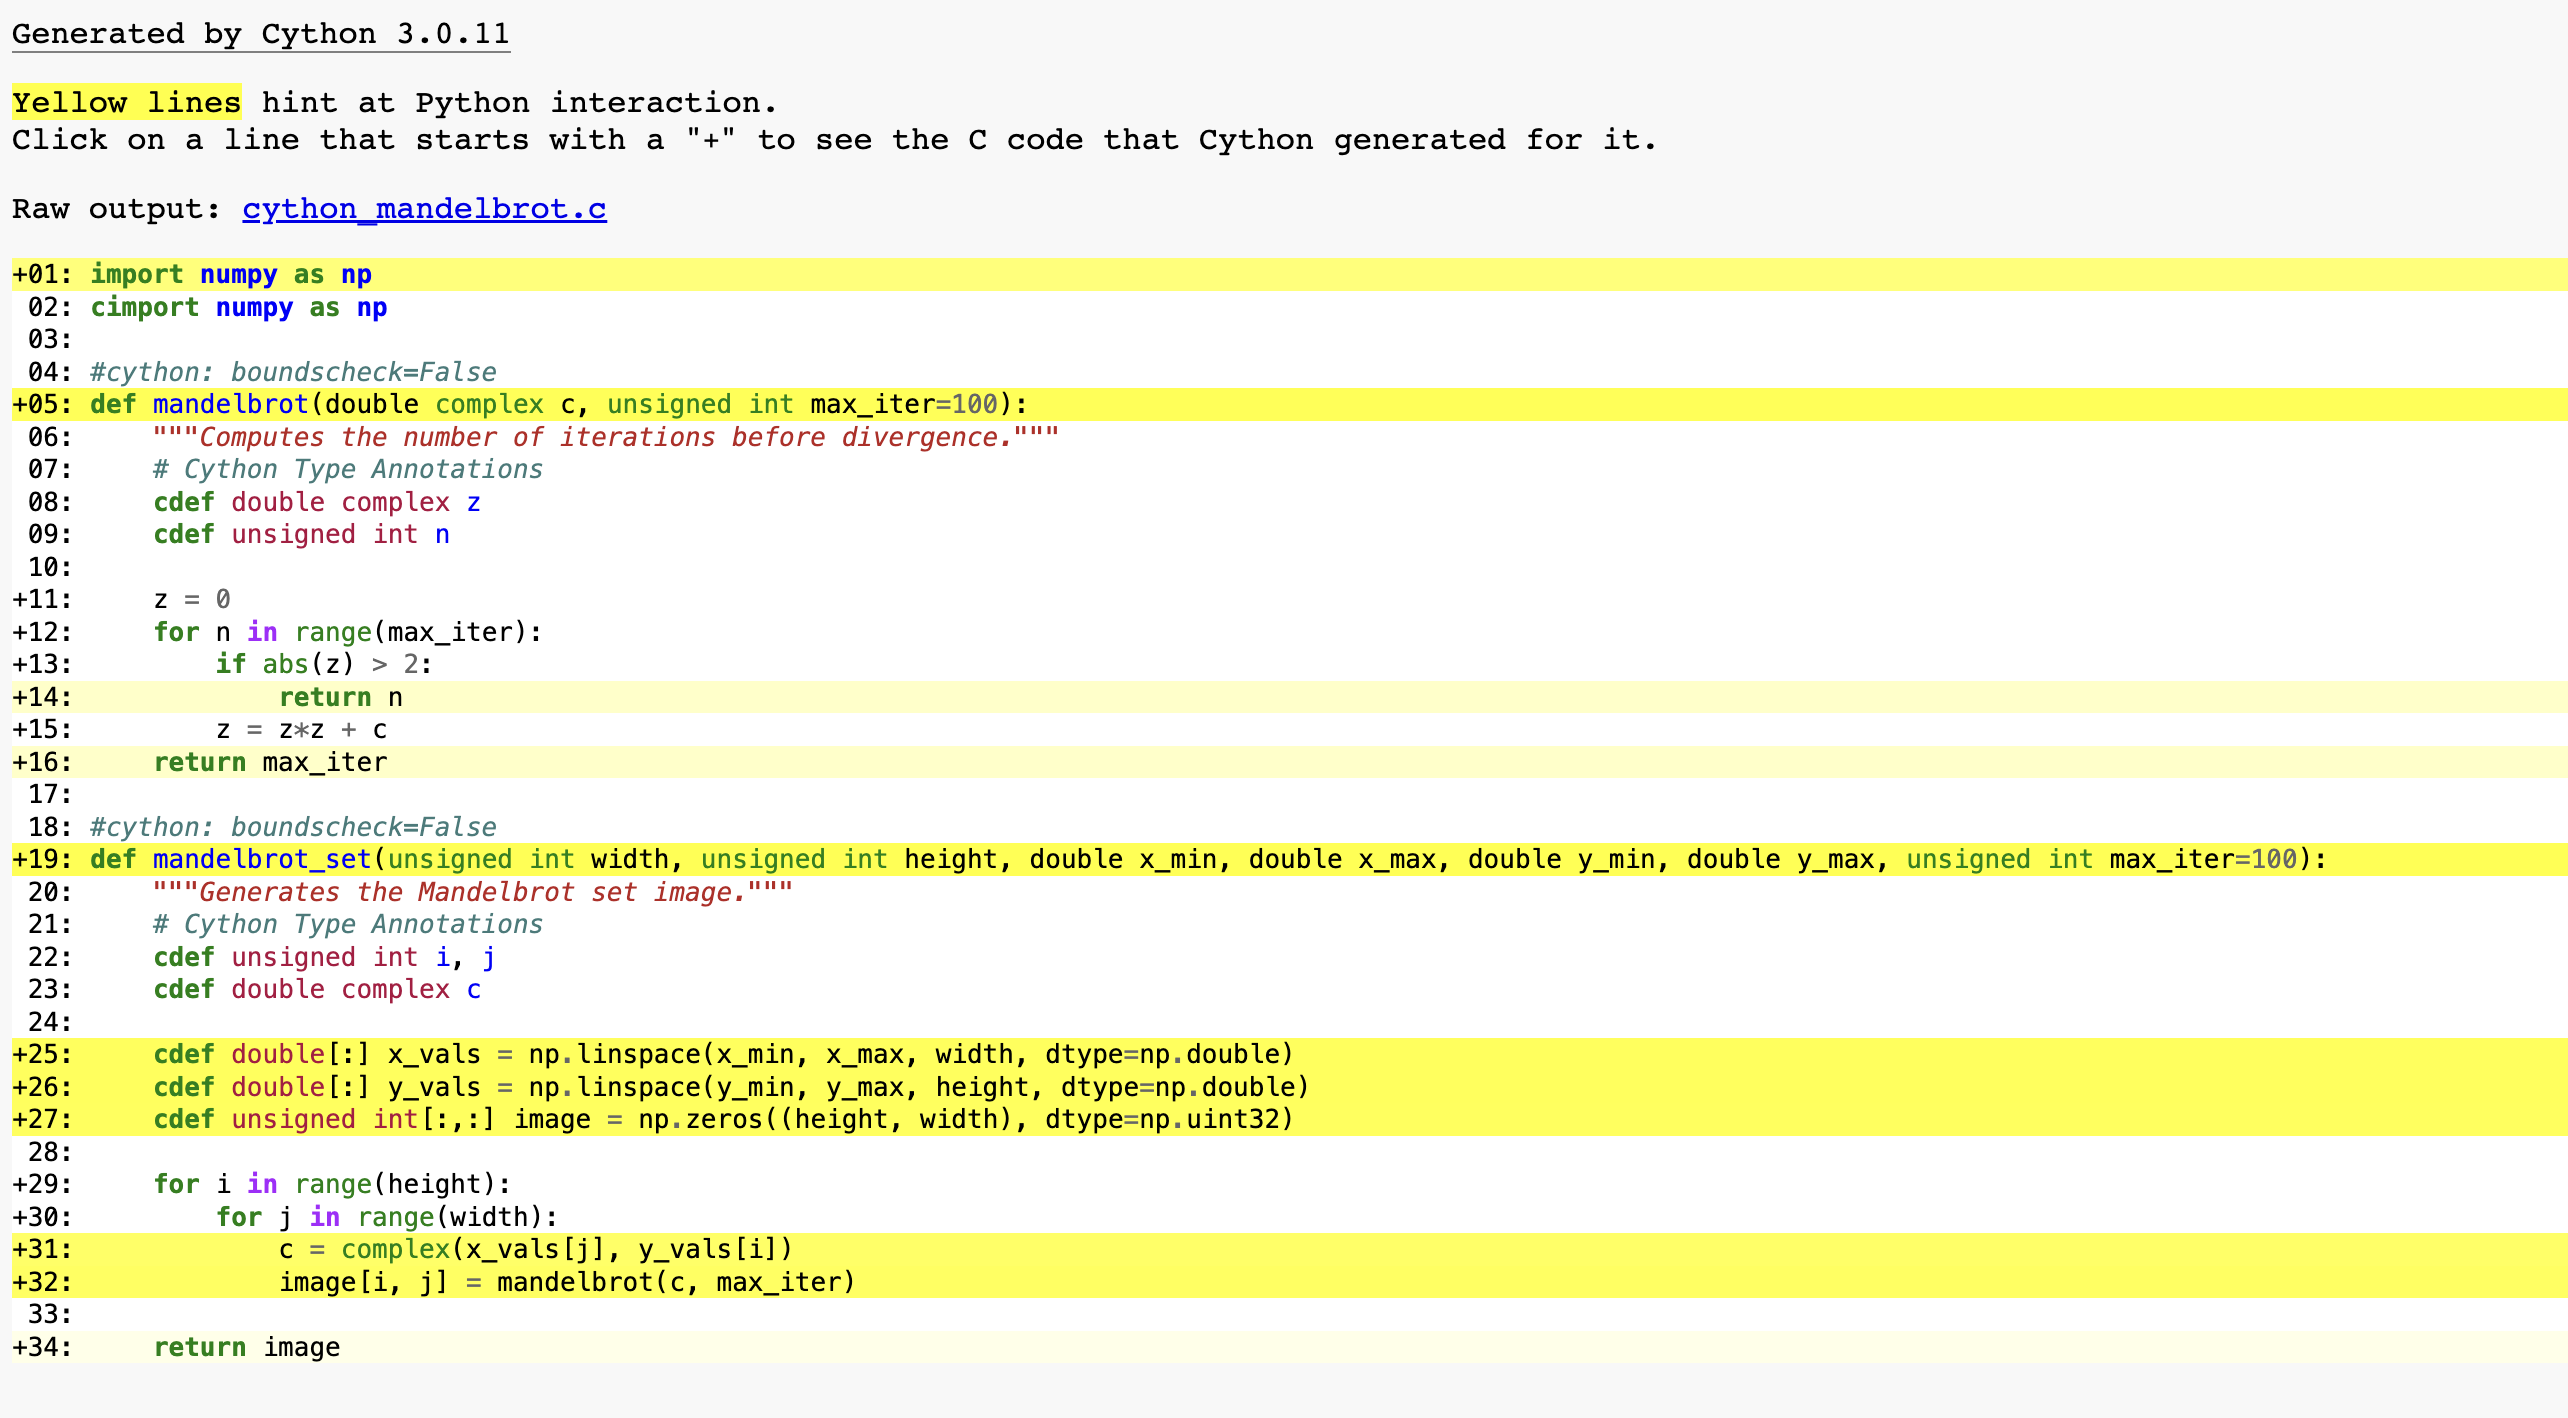
\includegraphics[width=0.8\textwidth]{images/after_annotate_mandelbrot.png}
  \caption{Python VM Calls in the Annotated Mandelbrot Code}
\end{figure}

Finally, we used the generated \verb|cython_mandelbrot| module above in the new Python file called \verb|mandelbrot_set_cython.py| (\href{https://github.com/paulmyr/DD2358-HPC25/blob/master/03_compgpu/bonus/mandelbrot_set_cython.py}{link}). To verify that our optimizations return answers that are consistent with the original implementation, we also implemented \verb|pytests| in a file (\href{https://github.com/paulmyr/DD2358-HPC25/blob/master/03_compgpu/bonus/mandelbrot_cython_default_test.py}{link}) for 4 different sizes of square grids, but using the same $x$ and $y$ coordinates that were provided with the original code. 

The result of the reduced calls to the Python VM because of our annotations can be seen in the HTML file above (\verb|cython_mandelbrot_after_annotate.html| is the name of the file in the code-repository), which was generated using the \verb|cython -a| command \textit{after} applying the annotations to the \verb|.pyx| file.

\subsubsection{Vectorization \& GPU Optimization of Baseline}
The vectorized version of the original Mandelbrot Set code can be found in the \verb|mandelbrot_torch.ipynb| notebook (\href{https://github.com/paulmyr/DD2358-HPC25/blob/master/03_compgpu/bonus/mandelbrot_torch.ipynb}{link}). Instead of using 2 functions, we now only use one function -- \verb|mandelbrot_set_torch| -- because of the vectorization. We used \underline{PyTorch} to run the Mandelbrot computation on the GPU. The comments of the function explain our reasoning for the vectorization. We used the \underline{T4 GPU} presented on Google Colab as our GPU for this section.

To get the \verb|x_vals| and \verb|y_vals| array as in the original code, we first used Numpy's \verb|linspace| method and then transformed that to a PyTorch tensor. This was required to ensure that we were able to correctly check the output of the vectorized code with the original output, and PyTorch's \verb|linspace| at times returned tensors with a higher precision than the ones returned by \verb|Numpy|: which at times caused difference in complex-number diversions. More specific information on this can be found in the comments in the notebook. 

As alluded to earlier, we have a \underline{Correctess Verification} section which checks the output of the vectorized version against that produced by the original Mandelbrot Set code using square grids of 4 sizes. This is not implemented as a Pytest, but rather a simple equality check. 

Finally, the notebook also compares the running time of the original code compared with the GPU version -- a plot of this along with specific timing info can be found at the end of the notebook. \\
\textit{Note: A comparison of all 3 implementations follows in the next section.}

\subsubsection{Comparison of the 3 Approaches}
To compare the running times of the 3 approaches, we used the code present in the \verb|mandelbrot_profile.py| file (\href{https://github.com/paulmyr/DD2358-HPC25/blob/master/03_compgpu/bonus/mandelbrot_profile.py}{link}). The running times for the PyTorch version of the original code were obtained on Google Colab T4 GPU and are the same as those present in the notebook mentioned in the section above. The Pure-Python (original) version and the Cython-ized version of the original code were both ran on an \underline{M1 MacBook Pro (16-inch, 2021)}. 

We measured the running times of each implementation on square grids of 4 sizes: $256 \times 246, 512 \times 512, 1024 \times 1024$ and $2048 \times 2048$. The $x$ and $y$ coordinates were the same ones present in the original Mandelbrot Set code. We took the average running time over 10 runs for a grid as the final running time of the Mandelbrot implemention for that grid. The maximum number of iterations was 100. 

Using this setup and approach, we obtained the following output on the terminal (the time below is in seconds): 

\begin{lstlisting}[language=bash,basicstyle=\tiny\ttfamily]
PROFILING COMPUTATION FOR default_generate (runs=10)
Avg Time for 256x256: 0.15021454157540576
Avg Time for 512x512: 0.5833664500853046
Avg Time for 1024x1024: 2.3403198414947837
Avg Time for 2048x2048: 9.467780166619923

PROFILING COMPUTATION FOR cython_generate (runs=10)
Avg Time for 256x256: 0.014089641778264194
Avg Time for 512x512: 0.055262112594209614
Avg Time for 1024x1024: 0.2187983958167024
Avg Time for 2048x2048: 0.8719794083852321

PROFILING COMPUTATION FOR torch_generate (runs=10) [-- taken from mandelbrot_torch.ipynb notebook]
Avg Time for 256x256: 0.012661022200018125
Avg Time for 512x512: 0.030808558399996855
Avg Time for 1024x1024: 0.10812428999999497
Avg Time for 2048x2048: 0.42733559330001186
\end{lstlisting}

The graphical version of the output is as follows (plotting the same times and grid sizes above in a $\log - \log$ plot)
\begin{figure}[H]
  \centering
  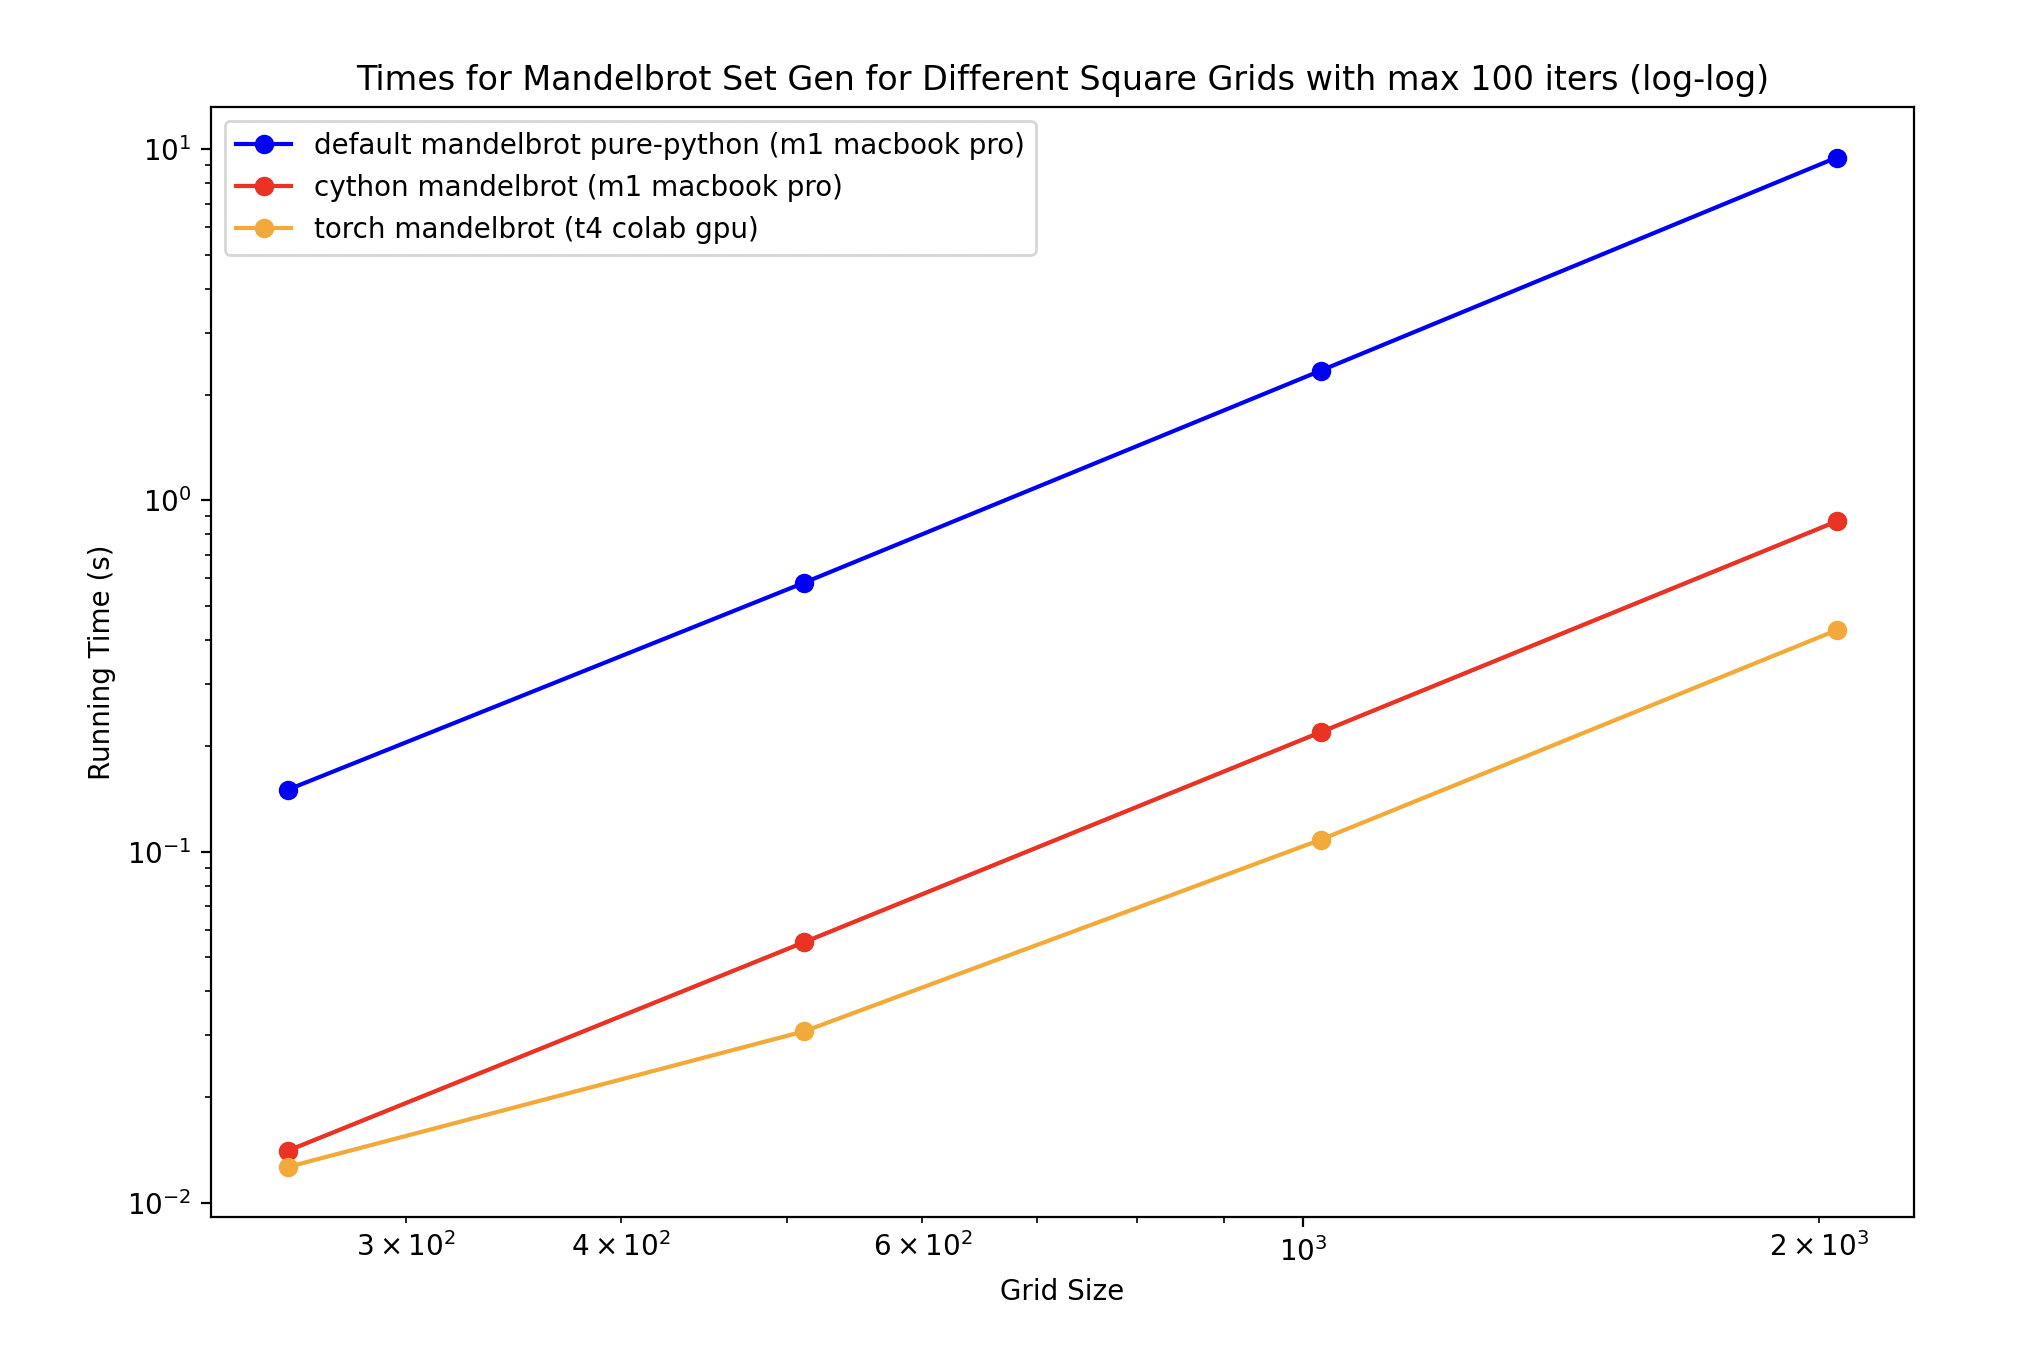
\includegraphics[width=0.8\textwidth]{images/bonus_comparison.png}
  \caption{Mandelbrot Set Running Time Comparisons For Different Grid Sizes}
\end{figure}

As can be seen from the figure above, the original (pure-python) version of the code is \underline{significantly slower} than the 2 optimized versions. In comparison, the Cython optimization of the original code is around \underline{10x faster}, and the Pytorch optimized version ran on the GPU is almost \underline{20x faster}. 

If we compare the Cython optimization of the original code to the PyTorch optimization (ran on the GPU), then the running times of the latter are \underline{almost 2x faster} than the former. This shows that vectorization and running the code on the GPU with PyTorch has noticeable benefits, but perhaps not as large a benefit as can be observed when comparing the PyTorch version with the pure-python (original implementation) version. The difference for the smallest grid ($256 \times 256$) also seems too small, but the 2x speedup starts becoming noticeable as the grid-sizes increase. 

Thus, if we were to make any conclusions from this experiment, we would say that if resources were available, then one should go for the \underline{vectorized version ran on the GPU} (what we call the PyTorch version in the report) for the Mandelbrot set. However, if a GPU isn't easily available, then the speedup given by Cython is also very significant when compared to the original, pure-python code. 

% \section{Appendix}

% content end
%###############################################################################

% TODO: bibliograpghy when needed
% \printbibliography

\end{document}
